\section{Metodología}
\label{sec:metodologia}

\subsection{Escenario y requisitos}
La Fig.~\ref{fig:escenario} muestra el escenario: el transmisor está montado sobre una banda transportadora accionada por un motor, cerca del tablero de contactores y del variador, y el receptor se ubica en la sala de supervisión. Si cien sensores reportan muestras de 16~bits a 10~Hz, la carga útil es 16~kb/s; con cabeceras y verificación de errores, $R_b=32$~kb/s deja un margen de 2:1. Se conservaron $R_s=32$~ksym/s y SPS~$=8$ porque cubren ese requerimiento, mantienen continuidad con la ficha de decisión y producen una tasa de banda base ($256$~kS/s) que se adapta a las tasas de los SDR con relaciones racionales sencillas.

\begin{figure}[H]
    \centering
    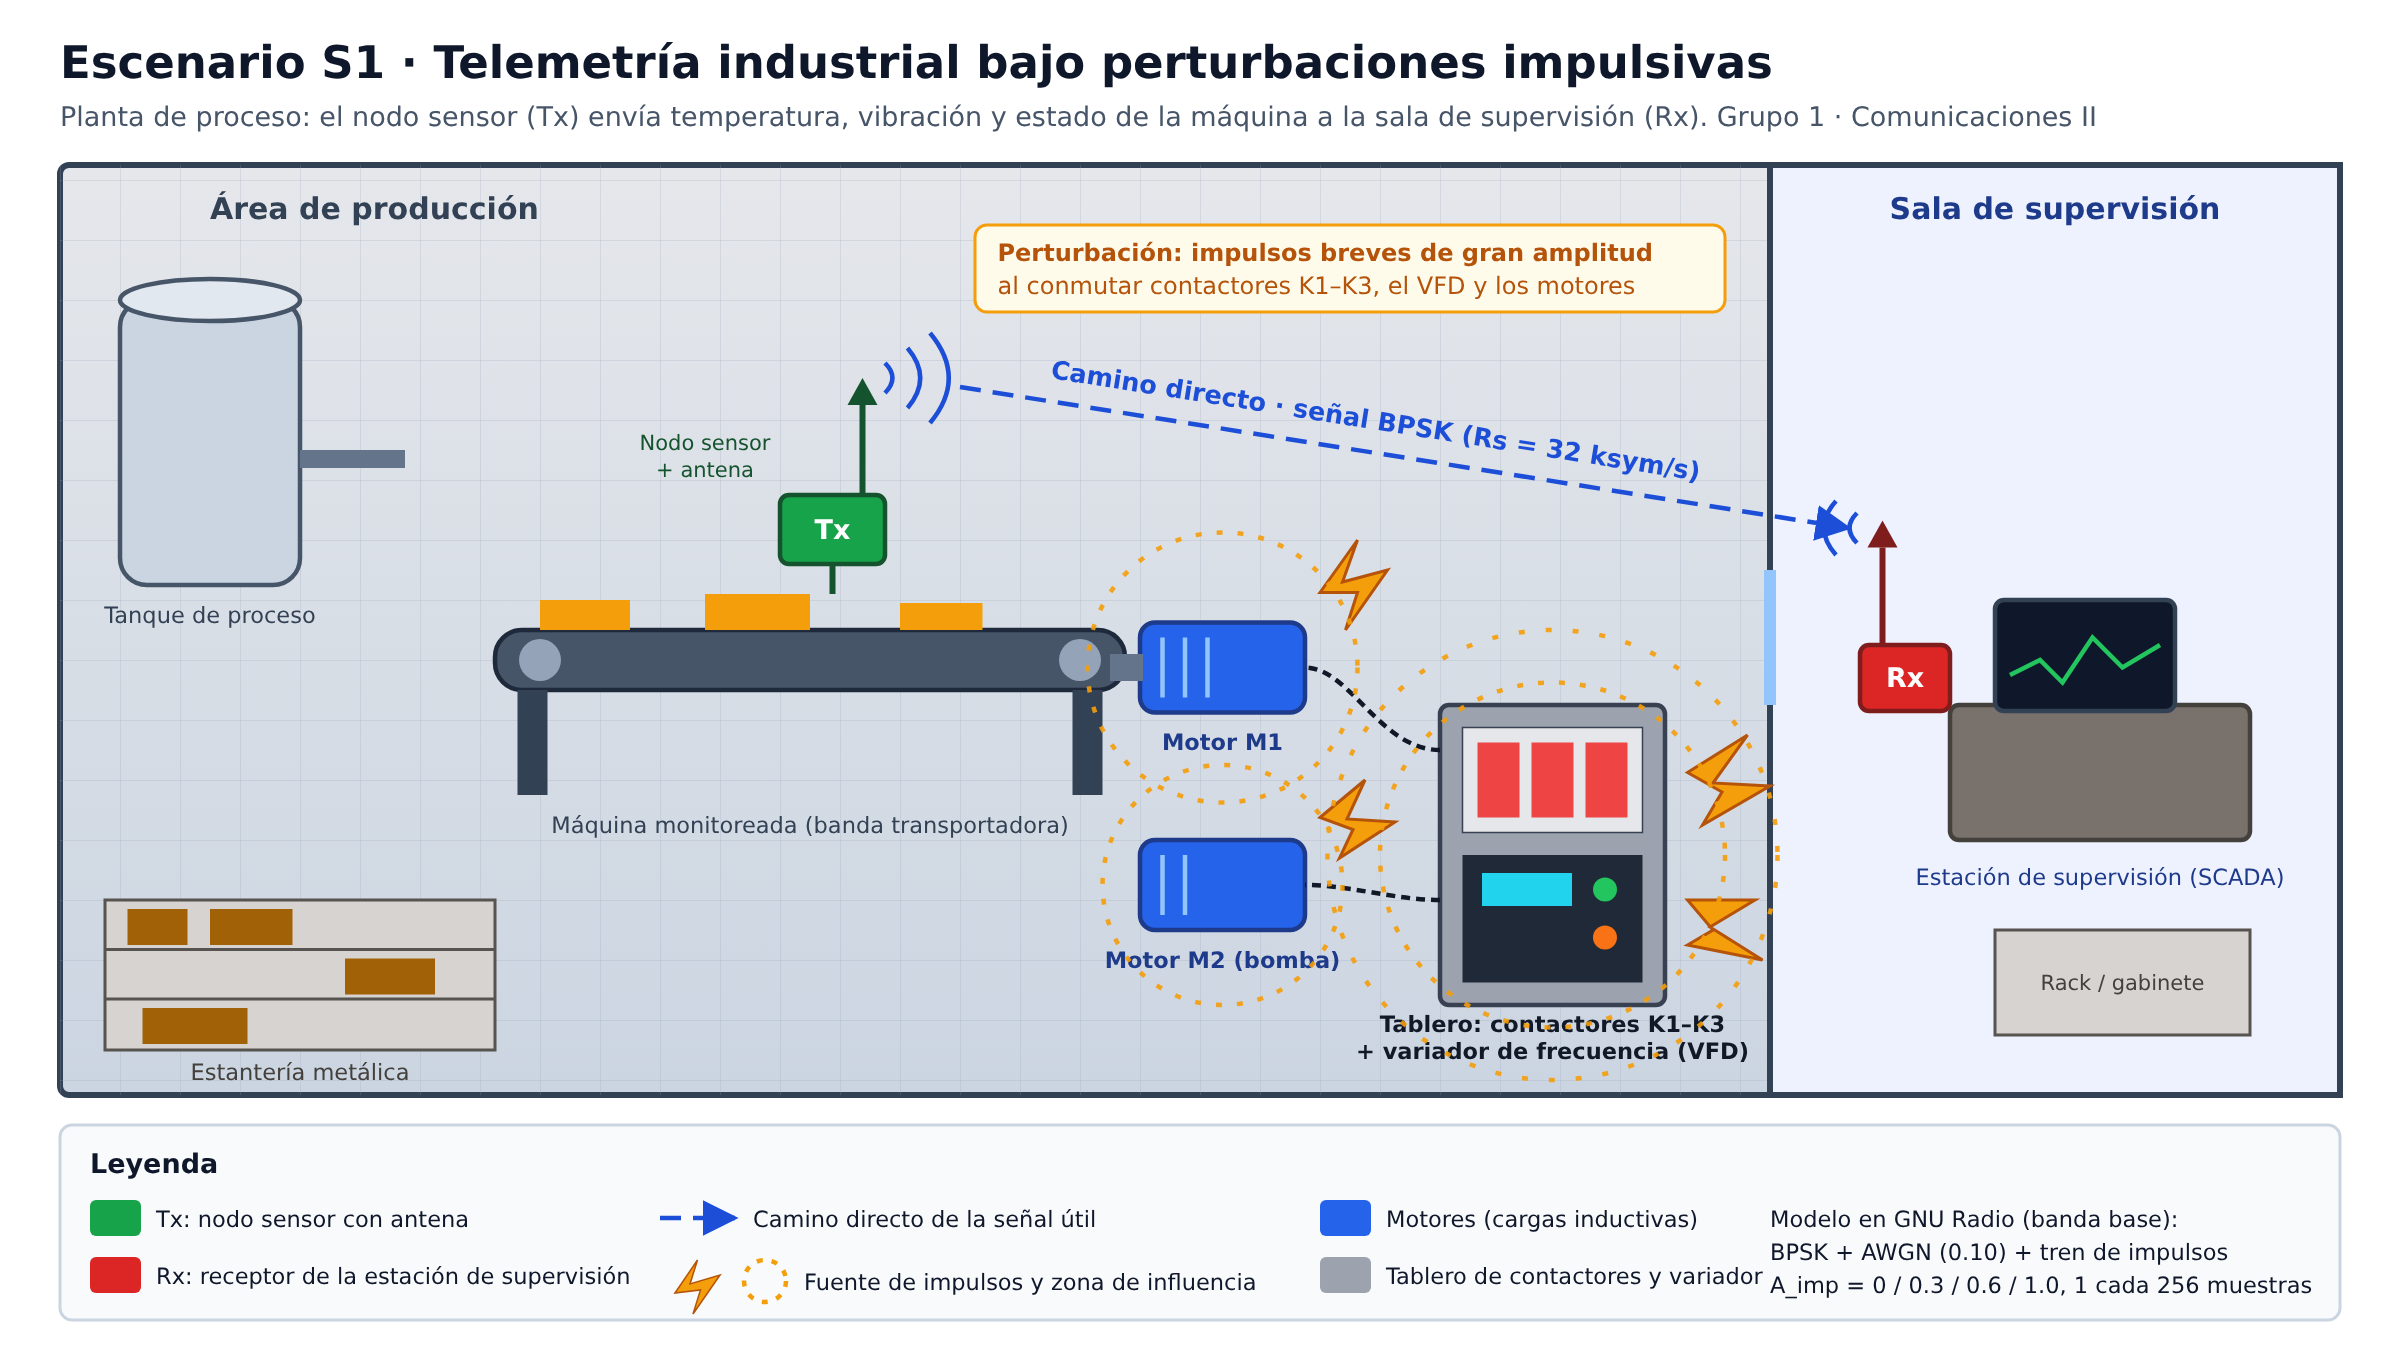
\includegraphics[width=\linewidth]{Figuras/escenario.png}
    \caption{Escenario contextual: nodo sensor (Tx), estación de supervisión (Rx) y fuentes de ruido impulsivo.}
    \label{fig:escenario}
\end{figure}

\subsection{Modelo del canal}
La señal recibida en banda base es
\begin{equation}
    r[n] = s[n] + w[n] + A_{imp}\sum_{k} \delta[n-255-256k],
    \label{eq:canal}
\end{equation}
donde $w[n]$ es AWGN complejo de potencia $0.10^2=0.01$. El tren de impulsos tiene potencia media $A_{imp}^2/256$, muy inferior a su potencia pico $A_{imp}^2$; este contraste explica gran parte de los resultados. Con la señal de potencia $\approx 1$, el AWGN equivale a $E_b/N_0\approx 29$~dB.

\subsection{Transmisor}
Se seleccionó BPSK ($M=2$, $k=\log_2 M=1$) porque, para una misma amplitud, ofrece la mayor distancia entre símbolos; se descartó OOK/ASK porque transporta la información en la amplitud, justamente lo que alteran los impulsos, y QPSK/16QAM porque aumentan $R_b$ sin necesidad y reducen la separación. Los bits provienen de una secuencia PRBS-15 conocida, se mapean como $0\rightarrow-1$, $1\rightarrow+1$ y se conforman con un filtro RRC de $\beta=0.35$ y longitud de 11 símbolos. La implementación genera $89$ coeficientes (número impar) con ganancia SPS, de modo que el nivel de cada símbolo es $\approx\pm1$. El ancho de banda ocupado es
\begin{equation}
    B \approx (1+\beta)R_s = 1.35\times 32~\text{kHz} = 43.2~\text{kHz},
    \label{eq:bw}
\end{equation}
frente a $\approx 64$~kHz entre primeros nulos del pulso rectangular usado en la fase de canal. La Tabla~\ref{tab:parametros} resume los parámetros.

\begin{table}[H]
    \centering
    \caption{Parámetros del enlace}
    \label{tab:parametros}
    \footnotesize
    \setlength{\tabcolsep}{4pt}
    \begin{tabular}{@{}lcc@{}}
        \toprule
        \textbf{Parámetro} & \textbf{Valor} & \textbf{Relación} \\
        \midrule
        Modulación & BPSK & $M=2$ \\
        Tasa de símbolos $R_s$ & 32 ksym/s & requisito \\
        Tasa de bits $R_b$ & 32 kb/s & $R_s\log_2 M$ \\
        Muestras por símbolo & 8 & -- \\
        Tasa de banda base & 256 kS/s & $R_s\cdot\text{SPS}$ \\
        Roll-off / span & 0.35 / 11 & -- \\
        Ancho de banda & 43.2 kHz & $(1+\beta)R_s$ \\
        AWGN del canal & 0.10 & $E_b/N_0\approx29$ dB \\
        Período de impulsos & 256 muestras & 1 ms \\
        \bottomrule
    \end{tabular}
\end{table}

\subsection{Receptor}
El receptor cumple cuatro funciones. \emph{Filtrado:} un filtro RRC acoplado con coeficientes $h_{rx}[n]=h[n]/\sum h^2$, de modo que la cascada Tx--Rx es un coseno alzado sin interferencia intersimbólica y el valor de decisión vale $\pm1$. \emph{Observación:} un diagrama de ojo a la salida del filtro acoplado. \emph{Muestreo:} cada filtro de 89 coeficientes introduce un retardo de 44 muestras; el retardo total es 88 muestras, exactamente 11 símbolos, por lo que se conserva una muestra de cada 8 con desfase 0, y la secuencia recuperada está retrasada 11 bits respecto a la transmitida. \emph{Decisión:} distancia mínima a los puntos $\pm1$, equivalente al umbral $I=0$.

El filtro acoplado también atenúa los impulsos: un impulso de una sola muestra aparece a la salida multiplicado por la forma del filtro, con un valor máximo
\begin{equation}
    \frac{\max_n h[n]}{\sum_n h^2[n]} = \frac{1.092}{7.94} = 0.137,
    \label{eq:atenuacion}
\end{equation}
de modo que un impulso de amplitud $A_{imp}$ desplaza la variable de decisión como máximo $0.137\,A_{imp}$.

\subsection{Implementación con SDR}
La Fig.~\ref{fig:sistema} muestra la arquitectura completa, implementada en un entorno de radio definida por software \cite{gnuradio,ortega2019}. Para hardware se conservan la modulación, $R_s$, SPS, $\beta$ y la decisión, y se agregan los parámetros propios del radio: frecuencia central $f_c=915$~MHz (banda ISM 902--928~MHz, sujeta a autorización del laboratorio), tasa del radio de 2~MS/s en HackRF One \cite{hackrf} y 1~MS/s en USRP \cite{uhd}, y remuestreo racional $256\,\text{k}\times125/16=2$~MS/s ($\times125/32$ para USRP), con la operación inversa en recepción. Los osciladores se sintonizan en $f_c\mp200$~kHz y la señal se desplaza digitalmente para alejarla de la componente de continua del conversor. Se eliminó el bloque de regulación de ritmo, porque el radio fija la tasa de muestras. Como los dos radios tienen osciladores independientes, el receptor de hardware agrega control automático de ganancia, un lazo de frecuencia de borde de banda, sincronización de reloj con banco polifásico de filtros RRC y un lazo de Costas de orden 2; para resolver la ambigüedad de fase de 180° se usa codificación diferencial.

\begin{figure*}[t]
    \centering
    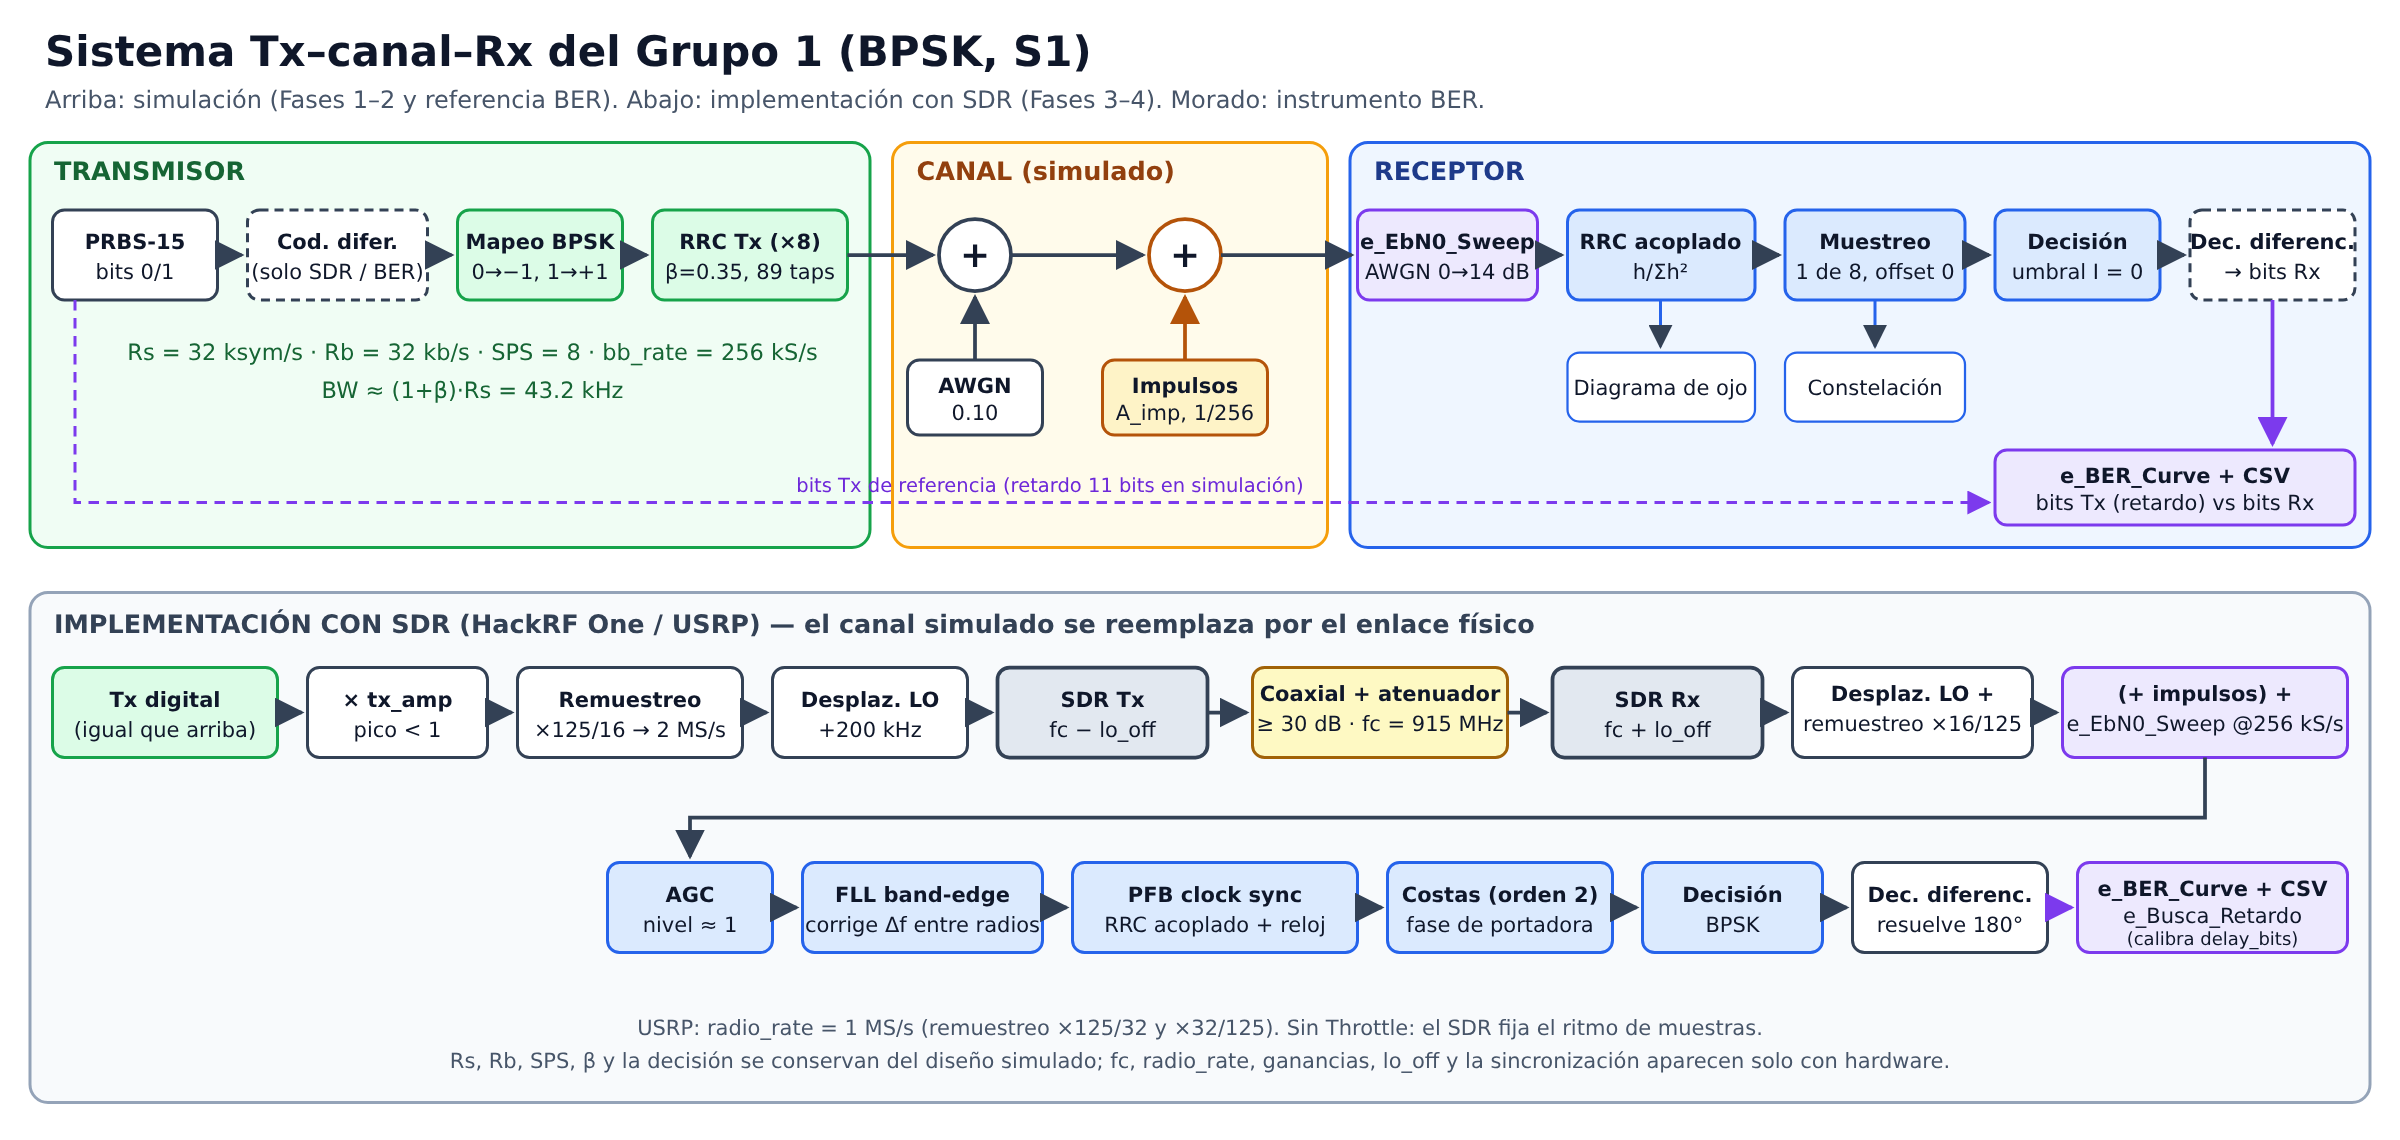
\includegraphics[width=0.92\textwidth]{Figuras/sistema_txrx.png}
    \caption{Arquitectura Tx--canal--Rx: simulación (arriba) e implementación con SDR (abajo), con el instrumento de medición BER.}
    \label{fig:sistema}
\end{figure*}

\subsection{Instrumentación BER}
Se integró el instrumento del curso: un bloque inserta AWGN controlado inmediatamente antes del receptor, con potencia
\begin{equation}
    P_n = \frac{P_s\,f_s}{R_b\,10^{(E_b/N_0)/10}},
    \label{eq:pn}
\end{equation}
y recorre $E_b/N_0$ de 0 a 14~dB en pasos de 1~dB, con $10^5$ bits por punto y $10^3$ bits de guarda; otro bloque compara los bits transmitidos (retrasados \texttt{delay\_bits}) con los recuperados y guarda la curva en un archivo CSV. Como referencia teórica se usa $P_b=Q\!\left(\sqrt{2E_b/N_0}\right)$ para BPSK y $P_b\approx2Q(1-Q)$ con codificación diferencial \cite{proakis2008}. Para calibrar \texttt{delay\_bits} en hardware se desarrolló un bloque que estima el retardo por correlación cruzada (Anexo~\ref{app:retardo}).
